\documentclass[11pt, twoside, pdftex]{article}

% This include all the settings that we should use for the document
\newcommand{\PDFTitle}{Using Library Modules in VHDL Designs}
\newcommand{\commonPath}{../../../Common}

\newcommand{\datePublished}{Mar 2022}

\newcommand{\versnum}{21.1} %version number quartus/AMP
\newcommand{\quartusname}{Quartus\textsuperscript{\textregistered} Prime}	
\newcommand{\textBar}{For \quartusname{} \versnum{}}
\newcommand{\thisyear}{2022 } %for copyright
\newcommand{\company}{FPGAcademy.org}
\newcommand{\longteamname}{FPGAcademy.org}
\newcommand{\teamname}{FPGAcademy}
\newcommand{\website}{FPGAcademy.org}

\newcommand{\productAcronym}{AMP}
\newcommand{\productNameShort}{Monitor Program}

\newcommand{\productNameMedTM}{Monitor Program}
\newcommand{\productNameMed}{Monitor Program}

%\newcommand{\headerLogoFilePath}[1]{#1/FPGAcademy.png}



\setlength\topmargin{-0.25in}
\setlength\headheight{0in}
\setlength\headsep{0.35in}
\setlength\textheight{8.5in}
\setlength\textwidth{7in}
\setlength\oddsidemargin{-0.25in}
\setlength\evensidemargin{-0.25in}
\setlength\parindent{0.25in}
\setlength\parskip{0in} 

\pdfpagewidth 8.5in
\pdfpageheight 11in

% listings is a package that supports encapsulating source code in LaTeX conveniently

\usepackage{listings}
% add support for graphics
\usepackage{graphicx}
\usepackage[usenames, dvipsnames]{color}

\def\expandparam\lstinputlisting[#1]#2{\edef\tmp{\noexpand\lstinputlisting[#1]{#2}}\tmp}

\widowpenalty 10000
\clubpenalty 10000

%%%%%%%%%%%%%%%%%%%% Source Code Formatting %%%%%%%%%%%%%%%%%%%%
\definecolor{globalCommentColour}{rgb}{0.588,0.588,0.588}

%%%%%%%%%%%%%%%%%%%%%%%%%%%%%%%%%%%%%%%%%%%%%%%%%%%%
% Defining a NiosII ASM highlighter for lstlisting
\lstdefinelanguage[NiosII]{Assembler} {
 	morekeywords={add, addi, and, andhi, andi, beq, bge, bgeu, bgt, bgtu, ble,  bleu, blt, bltu, bne, br, break,% 
 	bret, call, callr, cmpeq, cmpeqi, cmpge, cmpgei, cmpgeu, cmpgeui, cmpgt, cmpgti, cmpgtu, cmpgtui, cmple,%
 	cmplei, cmpleu, cmpleui, cmplt, cmplti, cmpltu, cmpltui, cmpne, cmpnei, custom, div, divu, eret, flushd,%
 	flushda, flushi, flushp, initd, initda, initi, jmp, jmpi, ldb, ldbio, ldbu, ldbuio, ldh, ldhio, ldhu, ldhuio,%
 	ldw, ldwio, mov, movhi, movi, movia, movui, mul, muli, mulxss, mulxsu, mulxuu, nextpc, nop, nor, or, orhi, ori,%
 	rdctl, rdprs, ret, rol, roli, ror, sll, slli, sra, srai, srl, srli, stb, stbio, sth, sthio, stw, stwio,%
 	sub, subi, sync, trap, wrctl, wrtcl, wrprs, xor, xori, xorhi, xori},% 	
 	morekeywords=[2]{.abort, .ABORT, .align, .app-file, .ascii, .asciz, .balign, .byte, .comm, .data, .def,%
 	.desc, .dim, .double, .eject, .else, .end, .endef, .endif, .equ, .equiv, .err, .extern, .file, .fill, .float,%
 	.global, .globl, .hword, .ident, .if, .include, .int, .irp, .irpc, .lcomm, .lflags, .line, .linkonce, .ln,%
 	.list, .long, .macro, .mri, .nolist, .octa, .org, .p2align, .psize, .quad, .rept, .sbttl, .scl, .section,%
 	.set, .short, .single, .size, .sleb128, .skip, .space, .stadb, .stabn, .stabs, .string, .symver, .tag,%
 	.text, .title, .type, .val, .uleb128, .word},% 	
 	morekeywords=[3]{et, bt, gp, sp, fp, ea, sstatus, ra, pc, status, estatus, bstatus, ienable, ipending, cpuid,%
 	exception, pteaddr, tlbacc, tlbmisc, eccinj, badaddr, config, mpubase, mpuacc},% 	
 	sensitive=t,%
 	alsoletter=.,%
	morestring=[b]",%
 	morecomment=[s]{/*}{*/},%
 	morecomment=[l]\#,%
   }[keywords,comments,strings]
   
   %% NOTE: morekeywords=[2] are GNU directives.
   
   \definecolor{niosInstructionColour}{rgb}{0.000,0.608,0.000}
   \definecolor{niosDirectiveColour}{rgb}{0.000,0.000,0.902}
   \definecolor{niosSpecialRegColour}{rgb}{0.000,0.000,0.000}
   \definecolor{niosStringColour}{rgb}{0.808,0.482,0.000}
   
   %% NOTE: To make bold use: =\bfseries\color{<colour>}
   \lstdefinestyle{defaultNiosStyle} {
   language=[NiosII]{Assembler},
   stringstyle=\color{niosStringColour},
   keywordstyle=\color{niosInstructionColour},
   keywordstyle=[2]\color{niosDirectiveColour},
   keywordstyle=[3]\itshape\color{niosSpecialRegColour}
   }
%%%%%%%%%%%%%%%%%%%%%%%%%%%%%%%%%%%%%%%%%%%%%%%%%%%%

%%%%%%%%%%%%%%%%%%%%%%%%%%%%%%%%%%%%%%%%%%%%%%%%%%%%
% Defining a ArmA9 ASM highlighter for lstlisting
\lstdefinelanguage[ArmA9]{Assembler} {
 	morekeywords={ADC, ADD, ADDS, AND, ANDS, B, BAL, BEQ, BGE, BGT, BL, BLT, BIC, BKPT, BLX, BNE, BX, CDP, CLZ, CMN, CMP, EOR,%
 	EORS, LDC, LDM, LDR, LDRB, LDRBT, LDRH, LDRSB, LDRSH, LDRT, LSL, MCR, MLA, MOV, MOVW, MOVT, MRC, MRS, MSR, MUL, MVN, ORR, PLD,%
 	ROR, RSB, RSC, SBC, SMLAL, SMULL, STC, STM, STR, STRB, STRBT, STRH, STRT, SUB, SUBS, SWI, SWP, SWPB, TEQ, UMLAL,
 	PUSH, POP, MOVS, RORS, LSR},%
 	morekeywords=[2]{.abort, .ABORT, .align, .app-file, .ascii, .asciz, .balign, .byte, .comm, .data, .def,%
 	.desc, .dim, .double, .eject, .else, .end, .endef, .endif, .equ, .equiv, .err, .extern, .file, .fill, .float,%
 	.global, .globl, .hword, .ident, .if, .include, .int, .irp, .irpc, .lcomm, .lflags, .line, .linkonce, .ln,%
 	.list, .long, .macro, .mri, .nolist, .octa, .org, .p2align, .psize, .quad, .rept, .sbttl, .scl, .section,%
 	.set, .short, .single, .size, .sleb128, .skip, .space, .stadb, .stabn, .stabs, .string, .symver, .tag,%
 	.text, .title, .type, .val, .vectors, .uleb128, .word},%
 	morekeywords=[3]{SP, PC, MIDR, CTR, TCMTR, TLBTR, MPIDR, ID_PFR0, ID_PFR1, ID_DFR0, ID_MMFR0, ID_MMFR1, ID_MMFR2,%
 	ID_MMFR3, ID_ISAR0, ID_ISAR1, ID_ISAR2, ID_ISAR3, ID_ISAR4, CCSIDR, CLIDR, AIDR, CSSELR, TTBR0, TTRB1, TTBR2, DACR,%
 	DFSR, IFSR, ADFSR, AIFSR, DFAAR, IFAR, ICIALLUIS, BPIALLIS, PAR, ICIALLU, ICIMVAU, BPIALL, DCIMVAC, DCISW, V2PCWPR,%
 	DCCVAC, DCCSW, DDIMVAC, DCISW, TLBALLIS, TLBIMVAIS, TLBIASIDIS, TLBIMVAAIS, TLBIALL, TLBIMVA, TLBIASID, TLBIMVAA,%
 	PMCR, PMCNTENSET, PMCNTENCLR, PMOVSR, PMSWINC, PMSELR, PMXEVTYPER, PMXEVCNTR, PMUSERENR, PMINTENSET, PMINTENCLR,%
 	PRRR, NRRR, PLEIDR, PLEASR, PLEFSR, PLEUAR, PLEPCR, VBAR, MVBAR, ISR, FCSEIDR, CONTEXTIDR, TPIDRURW, TPIDRURO, TPIDRPRW},%
 	sensitive=f,%
 	alsoletter=.,%
	morestring=[b]",%
 	morecomment=[s]{/*}{*/},%
 	morecomment=[l]{//},%
   }[keywords,comments,strings]
   
   %% NOTE: morekeywords=[2] are GNU directives.
   
   \definecolor{armInstructionColour}{rgb}{0.000,0.608,0.000}
   \definecolor{armDirectiveColour}{rgb}{0.000,0.000,0.902}
   \definecolor{armSpecialRegColour}{rgb}{0.000,0.000,0.000}
   \definecolor{armStringColour}{rgb}{0.808,0.482,0.000}
   
   \lstdefinestyle{defaultArmStyle} {
   language=[ArmA9]{Assembler},
   stringstyle=\color{armStringColour},
   keywordstyle=\color{armInstructionColour},
   keywordstyle=[2]\color{armDirectiveColour},
   keywordstyle=[3]\itshape\color{armSpecialRegColour}
   }
%%%%%%%%%%%%%%%%%%%%%%%%%%%%%%%%%%%%%%%%%%%%%%%%%%%%

%%%%%%%%%%%%%%%%%%%%%%%%%%%%%%%%%%%%%%%%%%%%%%%%%%%%
% Defining style for the verilog.

\definecolor{verilogCommentColour}{rgb}{0.000,0.502,0.000}

\lstdefinestyle{defaultVerilogStyle} {
language={Verilog},
keywordstyle=\color{blue},
commentstyle=\color{verilogCommentColour}
}
%%%%%%%%%%%%%%%%%%%%%%%%%%%%%%%%%%%%%%%%%%%%%%%%%%%%

%%%%%%%%%%%%%%%%%%%%%%%%%%%%%%%%%%%%%%%%%%%%%%%%%%%%
% Defining style for the vhdl.
\lstdefinestyle{defaultVHDLStyle} {
language={VHDL},
keywordstyle=\color{blue},
commentstyle=\color{verilogCommentColour}
}
%%%%%%%%%%%%%%%%%%%%%%%%%%%%%%%%%%%%%%%%%%%%%%%%%%%%

%%%%%%%%%%%%%%%%%%%%%%%%%%%%%%%%%%%%%%%%%%%%%%%%%%%%
% Java
\definecolor{javaStringColour}{rgb}{0.808,0.482,0}
%%%%%%%%%%%%%%%%%%%%%%%%%%%%%%%%%%%%%%%%%%%%%%%%%%%%

%%%%%%%%%%%%%%%%%%%%%%%%%%%%%%%%%%%%%%%%%%%%%%%%%%%%
% Defining language styles
% C
\definecolor{CStringColour}{rgb}{0.808,0.482,0}
%%%%%%%%%%%%%%%%%%%%%%%%%%%%%%%%%%%%%%%%%%%%%%%%%%%%

%%%%%%%%%%%%%%%%%%%%%%%%%%%%%%%%%%%%%%%%%%%%%%%%%%%%
% Defining extended LaTeX language.
\lstdefinelanguage[LocalLaTeX]{TeX}[LaTeX]{TeX}%
 	{moretexcs={bf, it, sf, lstset},%
   	}%

\lstdefinestyle{defaultLocalLatexStyle} {
language=[LocalLatex]{TeX},
keywordstyle=\color{blue}\bfseries,
keywordstyle=[2]\color{blue},
keywordstyle=[3]\color{blue}\bfseries
}
%%%%%%%%%%%%%%%%%%%%%%%%%%%%%%%%%%%%%%%%%%%%%%%%%%%%

\lstset{
%language = C,
%language = Verilog,
%basicstyle=\color{black}\rmfamily\ttfamily,
basicstyle=\small\color{black}\ttfamily,
commentstyle=\small\color{globalCommentColour}\itshape\ttfamily,
keywordstyle=\small\color{blue}\bfseries\ttfamily,
showstringspaces=false,
frame=none, %lines % boxed listings
breaklines=true,
breakatwhitespace=true,
tabsize=4
}
%%%%%%%%%%%%%%%%%%%%%%%%%%%%%%%%%%%%%%%%%%%%%%%%%%%%%%%%%%%%%%%%


%\usepackage[centering]{geometry}.
%%%%%%%%%%%%%%%%%%%%%%%%%%%%%%%%%%%%%%%%%%%%%%%%%%%
% Document Settings
\usepackage[labelsep=period]{caption}
% we can choose a better font later
%\usepackage{palatino}
\usepackage{fourier}
%\fontencoding{T1}
% include common used symbols
\usepackage{textcomp}
% add support for graphics
\usepackage{graphicx}
\usepackage[usenames, dvipsnames]{color}
% enable to draw thick or thin table hlines
\setlength{\doublerulesep}{\arrayrulewidth}
\usepackage{longtable}
\setlongtables
%\usepackage{array}
% It may be better to use PDFLaTeX as it can generate bookmarks for the
% document

% Add some useful packages
\usepackage{ae,aecompl}
\usepackage{epsfig,float,times}

% reset the font for section
\usepackage{sectsty}
%\allsectionsfont{\fontfamily{ptm}\selectfont}
\allsectionsfont{\usefont{OT1}{phv}{bc}{n}\selectfont}

% use compact space for sections
\usepackage[compact]{titlesec}
\titlespacing{\section}{0pt}{0.2in}{*0}
\titlespacing{\subsection}{0pt}{0.1in}{*0}
\titlespacing{\subsubsection}{0pt}{0.05in}{*0}

% fancyhdr header and footer customization
\usepackage{layout}
\usepackage{fancyhdr}
\pagestyle{fancy}
\fancyhead{}
\fancyhead[R]{\textit{\tiny{\textBar}}}
\fancyfoot{}
\fancyfoot[LO,
RE]{\textrm{\href{https://www.fpgacademy.org}{\small \longteamname}} \\ {\small \datePublished }}
\fancyfoot[RO, LE]{\small \thepage}
% two-side settings
%\fancyhead{} % clear all header fields
%\fancyfoot{} % clear all footer fields
%\fancyfoot[LE,RO]{\thepage}
\renewcommand{\headrulewidth}{2pt}
\renewcommand{\headrule}{{\color{blue} \hrule width\headwidth height\headrulewidth \vskip-\headrulewidth}}
\renewcommand{\footrulewidth}{0pt}

% Format the footer on page 1
\fancypagestyle{plain}{
\fancyhead{}
\fancyfoot{}
\fancyfoot[LO,
RE]{\textrm{\href{https://www.fpgacademy.org}{\small \longteamname}} \\ {\small \datePublished }}
\fancyfoot[RO, LE]{\small \thepage}
\renewcommand{\headrulewidth}{0pt}
}
% adjust some setting to try to make the figure stay in the same page with text
% Reference: 	http://www.cs.uu.nl/~piet/floats/node1.html
%   			http://mintaka.sdsu.edu/GF/bibliog/latex/floats.html
%   General parameters, for ALL pages:
\renewcommand{\topfraction}{0.9}	% max fraction of floats at top
\renewcommand{\bottomfraction}{0.8}	% max fraction of floats at bottom
%   Parameters for TEXT pages (not float pages):
\setcounter{topnumber}{3}
\setcounter{bottomnumber}{3}
\setcounter{totalnumber}{5}     % 2 may work better
\setcounter{dbltopnumber}{2}    % for 2-column pages
\renewcommand{\dbltopfraction}{0.9}	% fit big float above 2-col. text
\renewcommand{\textfraction}{0.07}	% allow minimal text w. figs
%   Parameters for FLOAT pages (not text pages):
\renewcommand{\floatpagefraction}{0.7}	% require fuller float pages
% N.B.: floatpagefraction MUST be less than topfraction !!
\renewcommand{\dblfloatpagefraction}{0.7}	% require fuller float pages
%%%%%%%%%%%%%%%%%%%%%%%%%%%%%%%%%%%%%%%%%%%%%%%%%%%
% remember to use [htp] or [htpb] for placement
%%%%%%%%%%%%%%%%%%%%%%%%%%%%%%%%%%%%%%%%%%%%%%%%%%%

% set no indent for paragraph
\setlength{\parindent}{0em}
\addtolength{\parskip}{11pt}
\newcommand{\compact}{[topsep=0pt]}
% use this package to reduce space
\usepackage{enumitem}
\usepackage{multirow}
\usepackage{rotating}
\usepackage{pifont}
\usepackage{dingbat}
\newcommand{\itemsecond}{$\circ$}
%
%%%%%%%%%%%%%%%%%%
\date{}
\author{}
%%%%%%%%%%%%%%%%%%
\newcommand{\de}{DE-series}
\newcommand{\up}{FPGAcademy}
\newcommand{\fabric}{Avalon Switch Fabric}
\newcommand{\TODO}[1]{\textcolor{red}{\textbf{TODO}: #1}}
\def\registered{{\ooalign{\hfil\raise .00ex\hbox{\scriptsize R}\hfil\crcr\mathhexbox20D}}}

% enable url and reference(bookmarks) in pdf
\usepackage{url}
\usepackage[pdftex, colorlinks]{hyperref}
\hypersetup{%
pdftitle={\PDFTitle},
linkcolor=blue,
hyperindex=true,
pdfauthor={\longteamname},
pdfkeywords={FPGAcademy, Academic Program, Example System},
bookmarksnumbered,
bookmarksopen=false,
filecolor=blue,
pdfstartview={FitH},
urlcolor=blue,
plainpages=false,
pdfpagelabels=true,
linkbordercolor={1 1 1} %no color for link border
}%
%%%%%%%%%%%%%%%%%%%%%%%%%%%%%%%%%%%%%%%%%%%%%%%%%%%
\setlength{\fboxsep}{0.7pt}
\setlength{\fboxrule}{0.5pt}

\newcommand{\red}[1]{{\color{red}\sf{#1}}}
\newcommand{\blue}[1]{{\color{blue}\sf{#1}}}




%%%%%%%%%%%%%%%%%%%%%%%%%
% Add title
\newcommand{\doctitle}{Using Library Modules \\ in VHDL Designs}
\newcommand{\dochead}{Using Library Modules in VHDL Designs}
% Usually no need to change these two lines
\title{\fontfamily{phv}\selectfont{\doctitle} }
\chead{ \small{\textsc{\bfseries \dochead} } }
% Customizations
%%%%%%%%%%%%%%%%%%%%%%%%%
% Allows multiple figures per page

\renewcommand\floatpagefraction{.9}
\renewcommand\topfraction{.9}
\renewcommand\bottomfraction{.9}
\renewcommand\textfraction{.1}   
\setcounter{totalnumber}{50}
\setcounter{topnumber}{50}
\setcounter{bottomnumber}{50}
\raggedbottom

%%%%%%%%%%%%%%%%%%
%%% DOCUMENT START
%\begin{document}
\begin{document}
\begin{table}
    \centering
    \begin{tabular}{p{5cm}p{4cm}}
        \hspace{-3cm}
        &
        \raisebox{1\height}{\parbox[h]{0.5\textwidth}{\Large\fontfamily{phv}\selectfont{\textsf{\doctitle}}}}
    \end{tabular}
    \label{tab:logo}
\end{table}

\colorbox[rgb]{0,0.384,0.816}{\parbox[h]{\textwidth}{\color{white}\textsf{\textit{\textBar}}}}

\thispagestyle{plain}
 
\section{Introduction}

This tutorial explains how Intel's library modules can be included in VHDL-based designs,
which are implemented by using the Quartus\textsuperscript{\textregistered} Prime software. 
\\
\\
{\bf Contents}:
\begin{itemize}
\item Example Circuit
\item Library of Parameterized Modules
\item Augmented Circuit with an LPM
\item Results for the Augmented Design
\end{itemize}
\clearpage
\newpage
\section{Background}

Practical designs often include commonly used circuit blocks
such as adders, subtractors, multipliers, decoders, counters, and shifters.
Intel provides efficient implementations of such blocks in the form
of library modules that can be instantiated in VHDL designs.
The compiler may recognize that a standard function specified in VHDL code
can be realized using a library module, in which case it may automatically
{\it infer} this module.
However, many library modules provide functionality that is too complex to be
recognized automatically by the compiler. These modules have to 
be instantiated in the design explicitly by the user. Quartus\textsuperscript{\textregistered} Prime software includes a 
{\it library of parameterized modules} ({\it LPM}).
The modules are general in structure and they are tailored to a specific
application by specifying the values of general parameters.

\noindent
Doing this tutorial, the reader will learn about:
\begin{itemize}
\item Library of parameterized modules (LPMs)
\item Configuring an LPM for use in a circuit
\item Instantiating an LPM in a designed circuit
\end{itemize}

\noindent
The detailed examples in the tutorial were obtained using the Quartus Prime version \versnum, 
but other versions of the software can also be used. When selecting a device within Quartus Prime, use the device names associated with FPGA chip on the DE-series board by referring to Table \ref{tab:device}. 

\begin{table}[H]
	\begin{center}
	\begin{tabular}{| c | c |}
	\hline
	Board & Device Name \\
	\hline
	DE0-CV & Cyclone\textsuperscript{\textregistered} V 5CEBA4F23C7 \\
	\hline
	DE0-Nano & Cyclone\textsuperscript{\textregistered} IVE EP4CE22F17C6 \\
	\hline
	DE0-Nano-SoC & Cyclone\textsuperscript{\textregistered} V SoC 5CSEMA4U23C6\\
	\hline
	DE1-SoC & Cyclone\textsuperscript{\textregistered} V SoC 5CSEMA5F31C6 \\
	\hline
	DE2-115 & Cyclone\textsuperscript{\textregistered} IVE EP4CE115F29C7 \\
	\hline
	DE10-Lite & Max\textsuperscript{\textregistered} 10 10M50DAF484C7G \\
	\hline
	DE10-Standard & Cyclone\textsuperscript{\textregistered} V SoC 5CSXFC6D6F31C6 \\
	\hline
	DE10-Nano & Cyclone\textsuperscript{\textregistered} V SE 5CSEBA6U2317 \\
	\hline
	\end{tabular}
	\caption{DE-series FPGA device names}
	\label{tab:device}
	\end{center}
\end{table}

\section{Example Circuit}

As an example, we will use the adder/subtractor circuit shown in Figure~\ref{fig:1}.
It can add, subtract, and accumulate $n$-bit numbers 
using the 2's complement number representation. 
The two primary inputs are numbers $A = a_{n-1} a_{n-2} \cdots a_0$
and $B = b_{n-1} b_{n-2} \cdots b_0$, and the primary output
is $Z = z_{n-1} z_{n-2} \cdots z_0$. Another input is the {\it AddSub} 
control signal which causes $Z = A + B$ to be performed when {\it AddSub} = 0 
and $Z = A - B$ when {\it AddSub} = 1.
A second control input, {\it Sel}, is used to select the accumulator mode of 
operation. If {\it Sel} = 0, the operation $Z = A \pm B$ is performed, but if
{\it Sel} = 1, then $B$ is added to or subtracted from the current
value of $Z$.
If the addition or subtraction operations result in arithmetic overflow, 
an output signal, {\it Overflow}, is asserted.

To make it easier to deal with asynchronous input signals, they are loaded 
into flip-flops on a positive edge of the clock. 
Thus, inputs $A$ and $B$ will be loaded into registers
{\it Areg} and {\it Breg}, while {\it Sel} and {\it AddSub} will be loaded into
flip-flops {\it SelR} and {\it AddSubR}, respectively.
The adder/subtractor circuit places the result into register {\it Zreg}.

\begin{figure}[H]
   \begin{center}
      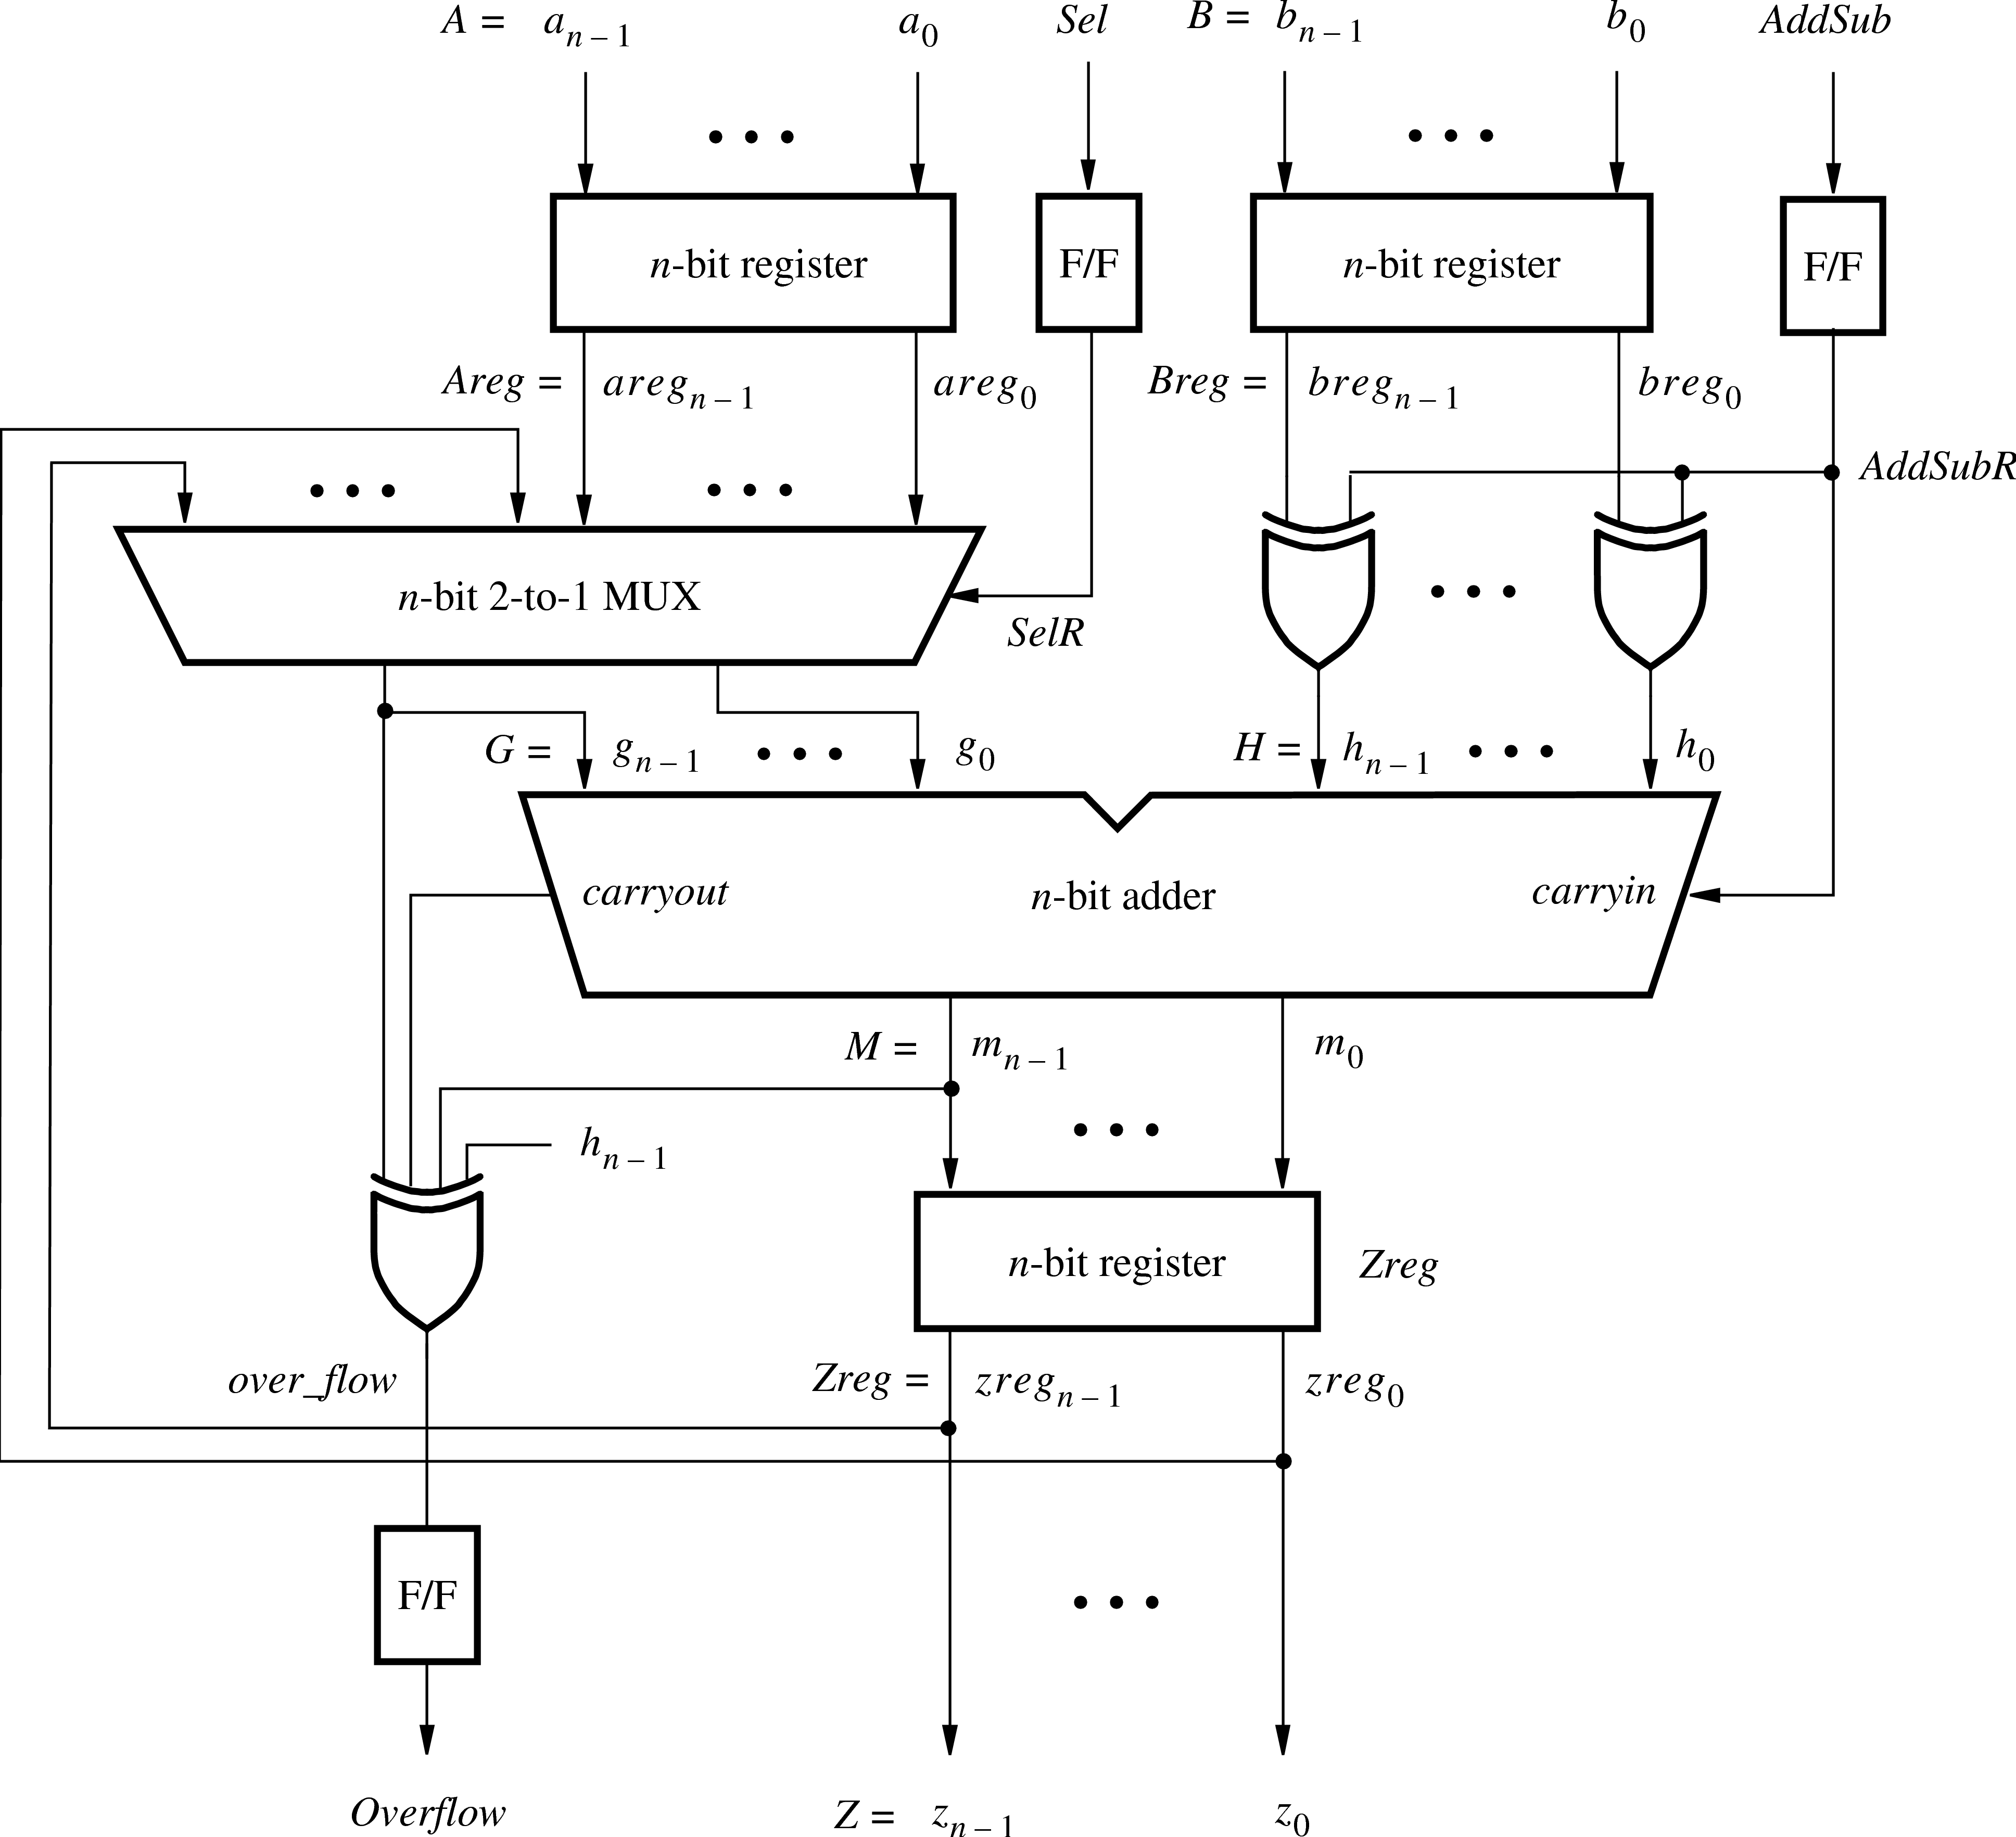
\includegraphics[scale=0.8]{figures/figure1.png}
   \caption{The adder/subtractor circuit.} 
	 \label{fig:1}
	 \end{center}
\end{figure} 

 
The required circuit is described by the VHDL code in Figure~\ref{fig:2}.
For our example, we use a 16-bit circuit as specified by $n = 16$.
Implement this circuit as follows:
\begin{itemize}
\item Create a project {\it addersubtractor}.
\item Include a file {\it addersubtractor.vhd}, which corresponds to Figure~\ref{fig:2},
in the project. 
%For convenience, this file is provided in the {\it design\_files} subdirectory within the tutorials folder, which is included on the
%CD-ROM that accompanies the DE-series board and can also be found on Altera's DE-series web pages. 
\item Select the FPGA chip that is on the DE-series board. A list of device names on DE-series boards can be found in Table \ref{tab:device}.
\item Compile the design.
\item Simulate the design by applying some typical inputs.
\end{itemize}

\newpage
\begin{figure}[H]

\lstinputlisting[language=VHDL, lastline=50]{design_files/addersubtractor.vhd}
	\caption{VHDL code for the circuit in Figure 1 (Part {\it a})}
	\label{fig:2}
\end{figure}
\newpage
\begin{center} %%%\begin{singlespace}

\lstinputlisting[language=VHDL, firstline=51]{design_files/addersubtractor.vhd}
Figure 2.  VHDL code for the circuit in Figure 1 (Part {\it b}).
\end{center}

\newpage
\section{Library of Parameterized Modules}

The LPMs in the IP Catalog are general in structure 
and they can be configured to suit a specific
application by specifying the values of various parameters.
We will use the {\it lpm\_add\_sub} module to simplify our 
adder/subtractor circuit defined in Figures~\ref{fig:1} and~\ref{fig:2}.
The augmented circuit is given in Figure~\ref{fig:3}. The {\it lpm\_add\_sub} module,
instantiated under the name {\it megaddsub},
replaces the adder circuit as well as the XOR gates that provide the input $H$
to the adder. Since arithmetic overflow is one of the outputs that the LPM
provides, it is not necessary to generate this output with a separate XOR gate.

To implement this adder/subtractor circuit, create a new directory named
{\it tutorial\_lpm}, and then create a project {\it addersubtractor2}.
Choose the same device as we previously selected (Refer to Table \ref{tab:device}) 
to allow a direct comparison of implemented designs.

\begin{figure}[H]
   \begin{center}
      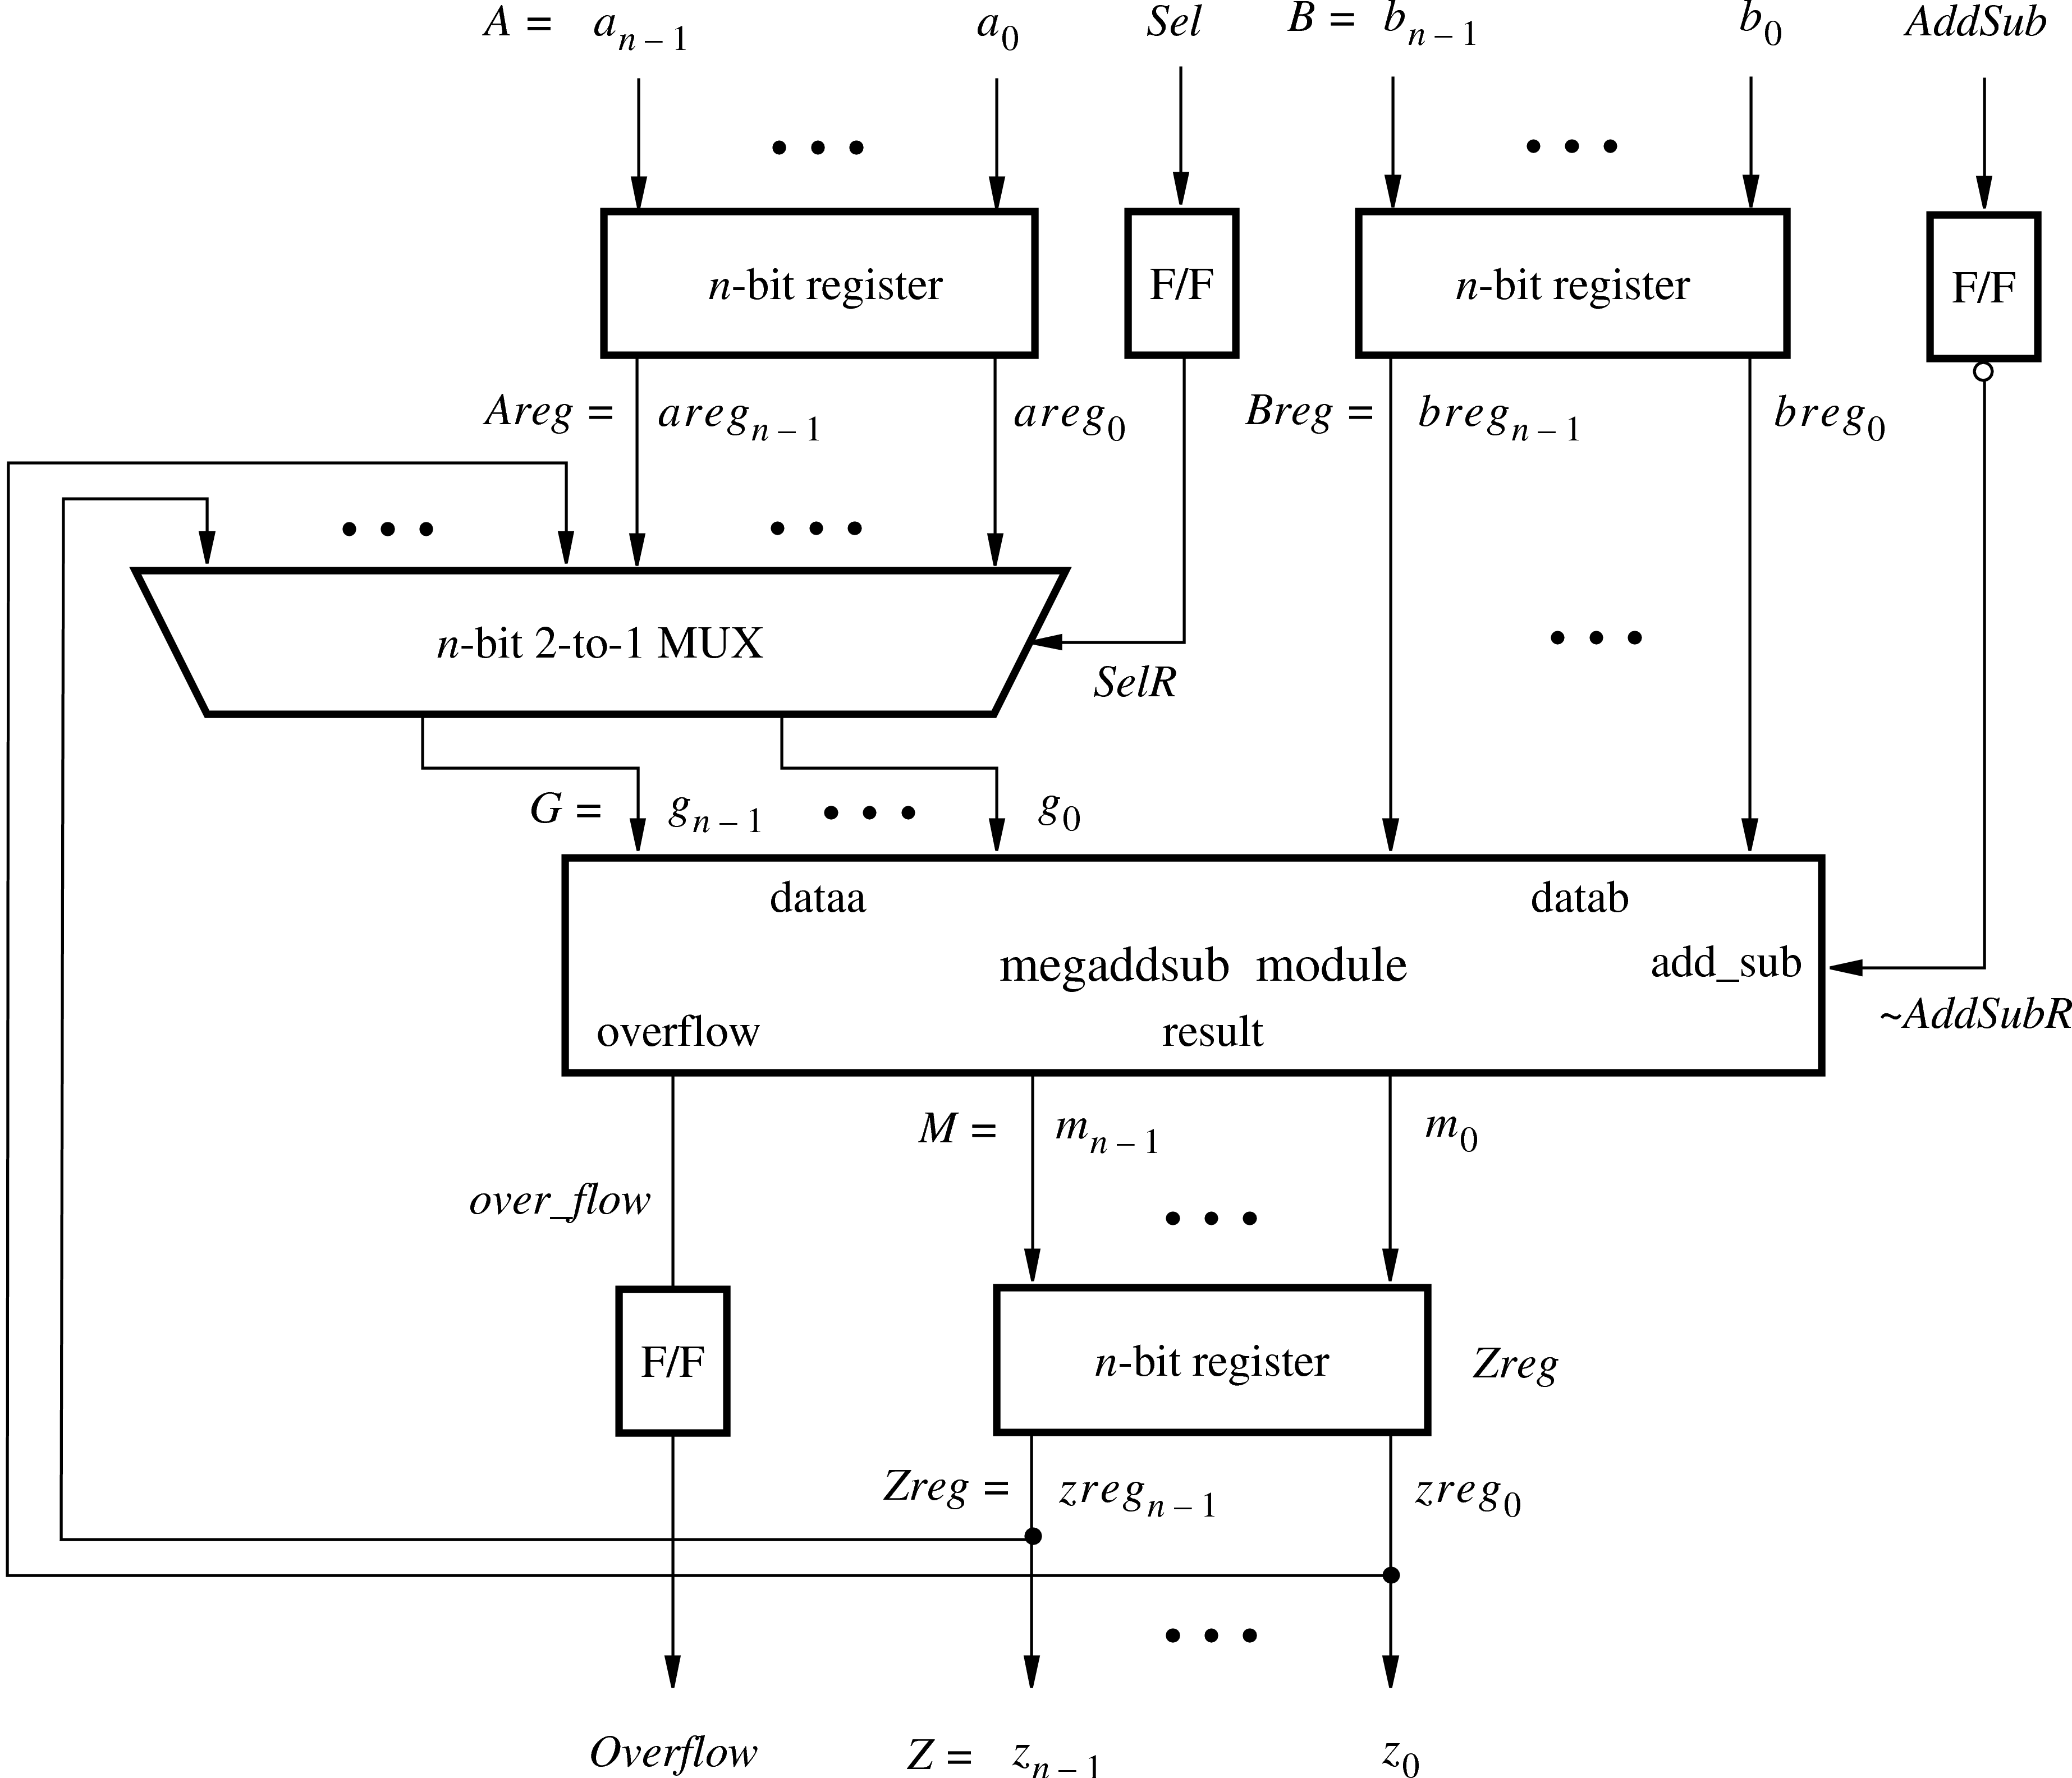
\includegraphics[scale=0.9]{figures/figure3.png}
   \caption{The augmented adder/subtractor circuit.} 
	 \label{fig:3}
	 \end{center}
\end{figure}  

The new design will include the desired LPM subcircuit specified as a VHDL
component that will be instantiated in the top-level VHDL design entity.
The VHDL component for the LPM subcircuit is generated by using a wizard as
follows:
\begin{enumerate}
\item Select {\sf Tools $>$ IP Catalog}, which
opens the IP Catalog window in Figure~\ref{fig:4}.
\item In the IP Catalog panel, expand {\sf Library $>$ Basic Functions $>$ Arithmetic} and double-click on {\sf LPM\_ADD\_SUB }


\begin{figure}[H]
   \begin{center}
      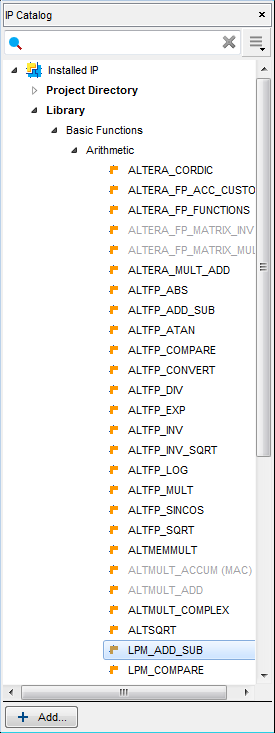
\includegraphics[scale=0.65]{figures/figure4.png}
   \caption{Choose an LPM.} 
	 \label{fig:4}
	 \end{center}
\end{figure} 
 
\begin{figure}[H]
   \begin{center}
      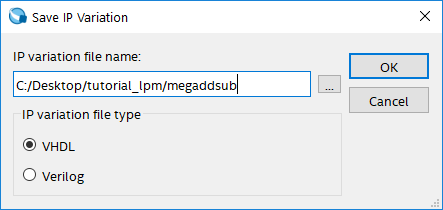
\includegraphics[scale=0.65]{figures/figure5.png}
   \caption{Create an LPM from the available library.} 
	 \label{fig:5}
	 \end{center}
\end{figure}  

\item In the pop-up box shown in Figure~\ref{fig:5}, choose {\sf VHDL} as the type of output file that should be created. 
The output file must be given a name; choose the name {\it megaddsub.vhd} and
indicate that the file should be placed in the directory 
{\it tutorial\_lpm} as shown in the figure. Press {\sf OK}.
 
\begin{figure}[H]
   \begin{center}
      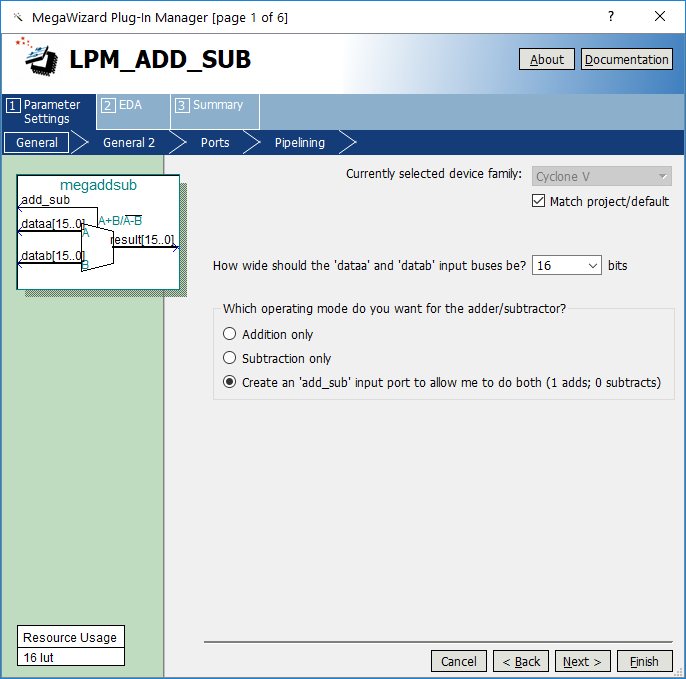
\includegraphics[scale=0.65]{figures/figure6.png}
   \caption{Specify the size of data inputs.} 
	 \label{fig:6}
	 \end{center}
\end{figure}  

\item In the box in Figure~\ref{fig:6} specify that the width of the data inputs is 16 bits.
Also, specify the operating mode in which one of the ports allows performing
both addition and subtraction of the input operand, under the control of 
the {\it add\_sub} input. A symbol for the resulting LPM is shown in the
top left corner. Note that if {\it add\_sub} = 1 then {\it result} = $A + B$;
otherwise, {\it result} = $A - B$. This interpretation of the control input
and the operation performed is different from our original design in 
Figures~\ref{fig:1} and~\ref{fig:2}, which we have to account for in the modified design.
Observe that we have included this change in the circuit in Figure~\ref{fig:3}.
Click {\sf Next}.
 
\begin{figure}[H]
   \begin{center}
      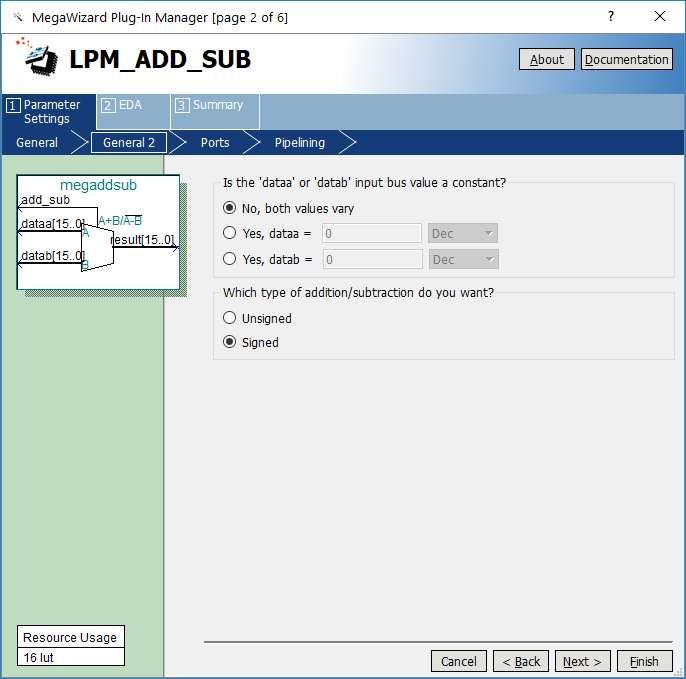
\includegraphics[scale=0.65]{figures/figure7.png}
   \caption{Further specification of inputs.} 
	 \label{fig:7}
	 \end{center}
\end{figure}

\item In the box in Figure~\ref{fig:7}, specify that the values of
both inputs may vary and select {\sf Signed} for the type of addition/subtraction.
Click {\sf Next}.

 
\begin{figure}[H]
   \begin{center}
      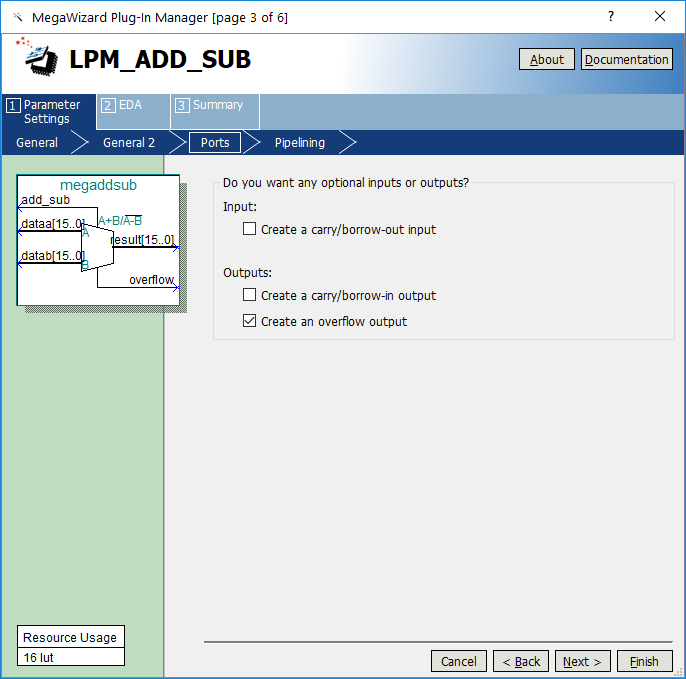
\includegraphics[scale=0.65]{figures/figure8.png}
   \caption{Specify the Overflow output.} 
	 \label{fig:8}
	 \end{center}
\end{figure}  

\item The box in Figure~\ref{fig:8} allows the designer to indicate optional inputs and 
outputs that may be specified. Since we need the overflow signal, make the 
{\sf Create an overflow output} choice and press {\sf Next}.
 
\begin{figure}[H]
   \begin{center}
      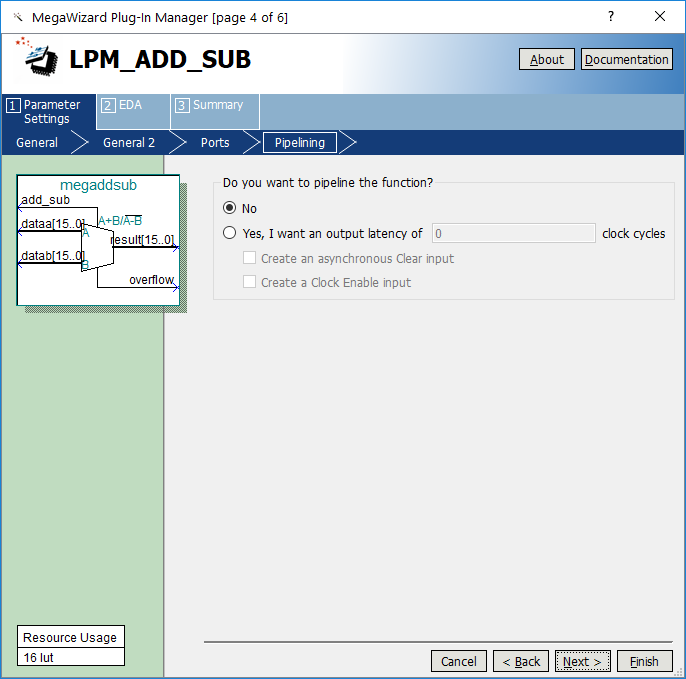
\includegraphics[scale=0.65]{figures/figure9.png}
   \caption{Refuse the pipelining option.} 
	 \label{fig:9}
	 \end{center}
\end{figure} 

\item In the box in Figure~\ref{fig:9} say {\sf No} to the pipelining option and 
click {\sf Next}.

\item Figure~\ref{fig:10} shows the simulation model files needed to simulate the generated design. Press {\sf Next} to proceed to the final page.

\begin{figure}[H]
   \begin{center}
      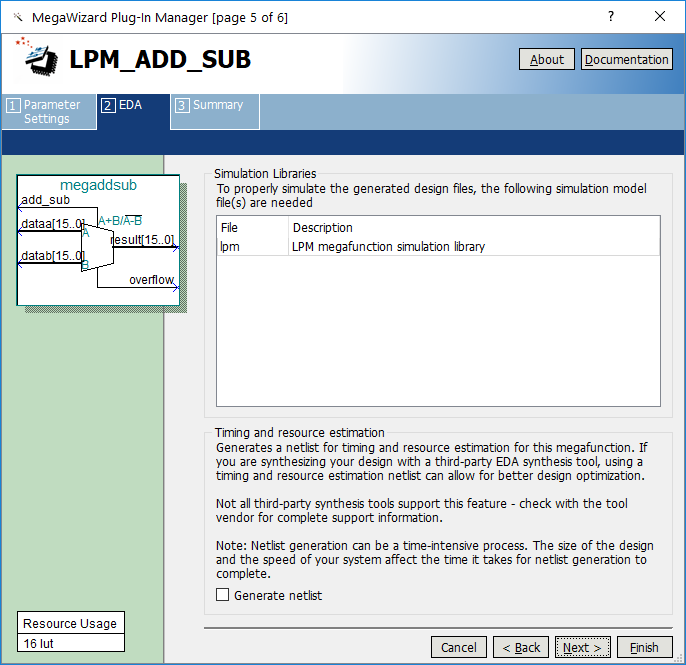
\includegraphics[scale=0.65]{figures/figure10.png}
   \caption{Simulation model files.} 
	 \label{fig:10}
	 \end{center}
\end{figure}

\item Figure~\ref{fig:11} gives a summary which shows the files that the wizard will create.
Press {\sf Finish} to complete the process.

\begin{figure}[H]
   \begin{center}
      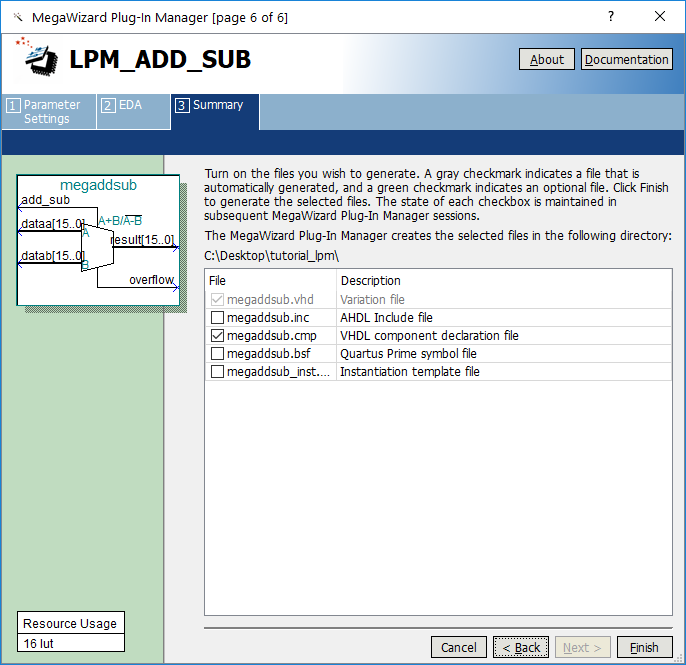
\includegraphics[scale=0.55]{figures/figure11.png}
   \caption{Files created by the wizard.}
	 \label{fig:11}
	 \end{center}
\end{figure} 

\item The box in Figure~\ref{fig:12} may pop up. If it does, make sure to press {\sf No}, since
adding the newly generated files to the project is not needed when using VHDL (in fact,
this may cause compilation errors).

\begin{figure}[H]
   \begin{center}
      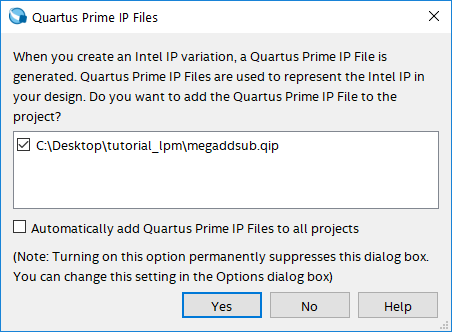
\includegraphics[scale=0.50]{figures/figure12.png}
   \caption{Do not add the new files to the project.} 
	 \label{fig:12}
	 \end{center}
\end{figure}  

\end{enumerate}

\section{Augmented Circuit with an LPM}

We will use the file {\it megaddsub.vhd} in our modified design.
Figure~\ref{fig:13} depicts the VHDL code in this file; note that we have not shown 
the comments in order to keep the figure small.

\begin{figure}[H]

\lstinputlisting[language=Verilog, xleftmargin=1cm]{design_files/megaddsub.v}
	\caption{Verilog code for the ADD\_SUB LPM.}
	\label{fig:13}
\end{figure}

The modified VHDL code for the adder/subtractor design is given in Figure~\ref{fig:14}.
It incorporates the code in Figure~\ref{fig:13} as a component. Put this code into a file
{\it addersubtractor2.vhd} under the directory {\it tutorial\_lpm}.  Also make sure to change the top level entity by selecting Project -> set as top level entity.
The key differences between this code and Figure~\ref{fig:2} are:
\begin{itemize}
\item The statements that define the {\it over\_flow} signal 
and the XOR gates (along with the signal H) are no longer needed.
\item The {\it adderk} entity, which specifies the adder circuit, is replaced 
by {\it megaddsub} entity. Note that the {\it dataa} and {\it datab} inputs shown 
in Figure~\ref{fig:6} are driven by the $G$ and {\it Breg} vectors, respectively.
\item {\it AddSubR} signal is specified to be the inverted version of the {\it AddSub}
signal to conform with the usage of this control signal in the LPM.
\end{itemize}
\begin{figure}[H]

\lstinputlisting[language=Verilog, lastline=33, xleftmargin=2cm]{design_files/addersubtractor2.v}
	\caption{Verilog code for the circuit in Figure 3 (Part {\it a})}
	\label{fig:14}
\end{figure}
\newpage
\begin{center} %%%\begin{singlespace}

\lstinputlisting[language=Verilog, firstline=34, xleftmargin=2cm]{design_files/addersubtractor2.v}
Figure 14.  Verilog code for the circuit in Figure 3 (Part {\it b}).
\end{center}

\newpage
\begin{center} %%%\begin{singlespace}

\lstinputlisting[language=VHDL, firstline=80]{design_files/addersubtractor2.vhd}  
Figure 14.  VHDL code for the circuit in Figure 3 (Part {\it c}).
\end{center}


Ensure {\it addersubtractor2.vhd} has been included in the project. To do so,
select {\sf Project $>$ Add/Remove Files in Project} to reach the window in Figure~\ref{fig:15}.
If the file {\it addersubtractor2.vhd} is not already listed as being included 
in the project, browse for the available files by clicking the button
{\sf ...} to reach the window in Figure~\ref{fig:16}.
Select the file {\it addersubtractor2.vhd} and click {\sf Open}, which returns to the
window in Figure~\ref{fig:15}. Click {\sf Add} to include the file and then click {\sf OK}.
Now, the modified design can be compiled and simulated in the usual way.

\begin{figure}[H]
   \begin{center}
      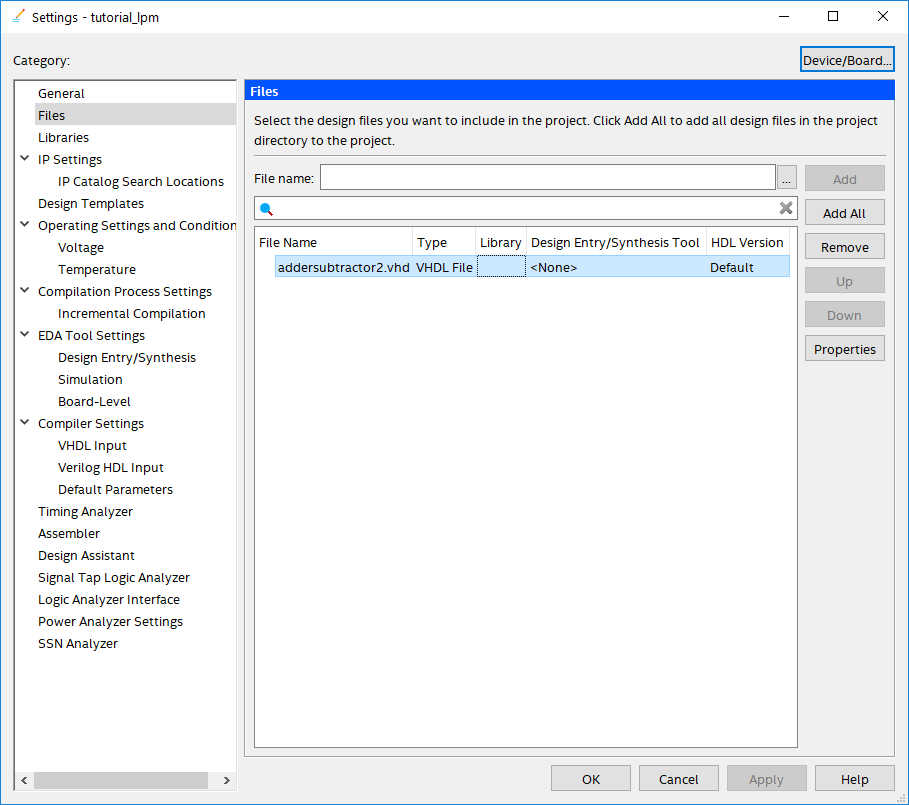
\includegraphics[scale=0.65]{figures/figure15.png}
   \caption{Inclusion of the new file in the project.} 
	 \label{fig:15}
	 \end{center}
\end{figure}
 
\begin{figure}[H]
   \begin{center}
      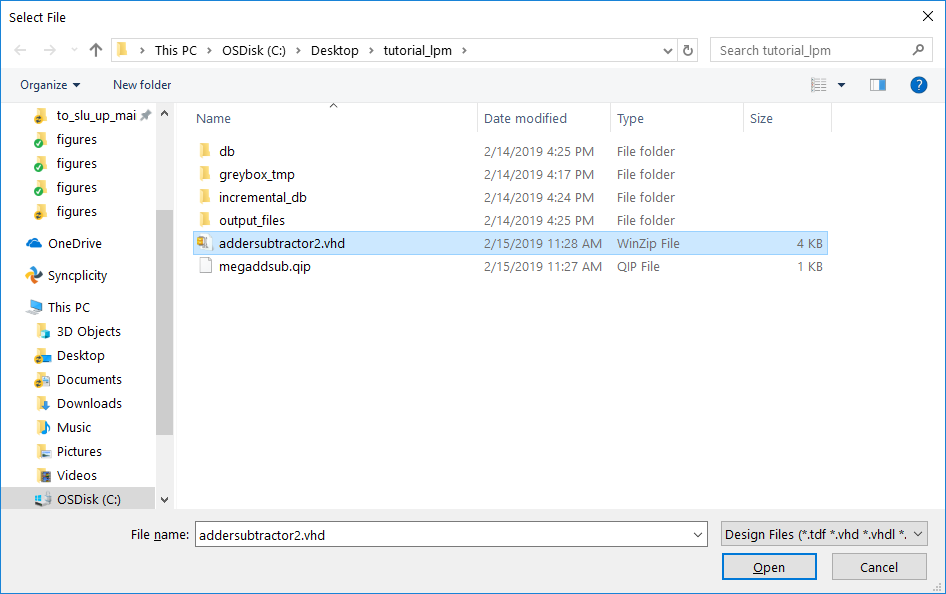
\includegraphics[scale=0.65]{figures/figure16.png}
   \caption{Specify the {\it addersubtractor2.vhd} file.} 
	 \label{fig:16}
	 \end{center}
\end{figure} 

\newpage
\section{Results for the Augmented Design}

Compile the design and look at the summary, which is depicted in Figure~\ref{fig:17}.
Observe that the modified design is implemented with a similar number of logic elements
compared to using the code in Figure~\ref{fig:2}.
 
\begin{figure}[H]
   \begin{center}
      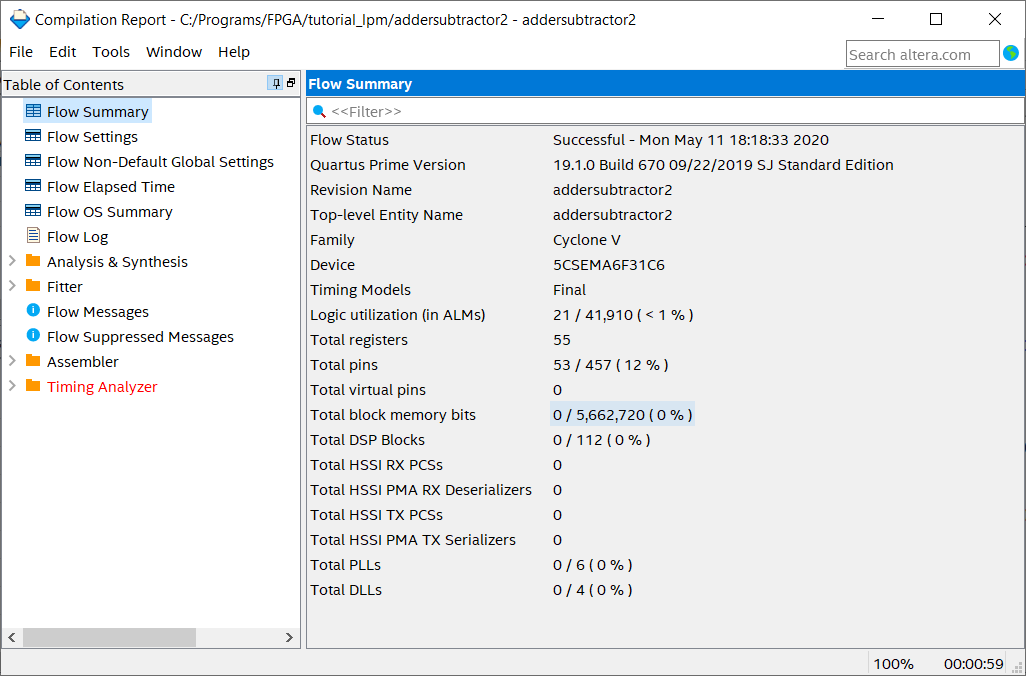
\includegraphics[scale=0.70]{figures/figure17.png}
   \caption{Compilation Results for the Augmented Circuit.} 
	 \label{fig:17}
	 \end{center}
\end{figure} 

 
% Copyright and Trademark

%\newcommand{\datePublished}{Mar 2022}

\newcommand{\versnum}{21.1} %version number quartus/AMP
\newcommand{\quartusname}{Quartus\textsuperscript{\textregistered} Prime}	
\newcommand{\textBar}{For \quartusname{} \versnum{}}
\newcommand{\thisyear}{2022 } %for copyright
\newcommand{\company}{FPGAcademy.org}
\newcommand{\longteamname}{FPGAcademy.org}
\newcommand{\teamname}{FPGAcademy}
\newcommand{\website}{FPGAcademy.org}

\newcommand{\productAcronym}{AMP}
\newcommand{\productNameShort}{Monitor Program}

\newcommand{\productNameMedTM}{Monitor Program}
\newcommand{\productNameMed}{Monitor Program}

%\newcommand{\headerLogoFilePath}[1]{#1/FPGAcademy.png}



%%%%%%%%%%%%%%%%%%%%%%%%%%%%%%%%%%%%%%%%
%%% FPGAcademy Copyright Information %%%
%%%%%%%%%%%%%%%%%%%%%%%%%%%%%%%%%%%%%%%%

%Always put the copyright on a new page (clear page), with some vertical space from top
\clearpage
\vspace{1in}

\noindent

Copyright {\copyright} FPGAcademy.org. All rights reserved. FPGAcademy and the FPGAcademy logo are trademarks of  FPGAcademy.org.  This document is being provided on an ``as-is'' basis and as an accommodation and therefore all warranties, representations or guarantees of any kind (whether express, implied or statutory) including, without limitation, warranties of merchantability, non-infringement, or fitness for a particular purpose, are specifically disclaimed.

%FPGAcademy assumes no responsibility or liability arising out of the application or use of any information,  product,  or  service  described  herein  except  as  expressly  agreed  to  in  writing  by  FPGAcademy.



**Other names and brands may be claimed as the property of others.




\end{document}
